\documentclass[dvips,landscape]{foils}
\usepackage{graphicx,psfrag}
\input defs.tex
\raggedright
\special{! TeXDict begin /landplus90{true}store end }
\renewcommand{\oursection}[1]{
\foilhead[-1.0cm]{#1}
}

\title{Stochastic Subgradient Method}
\author{}
\MyLogo{Prof.\ S.\ Boyd, EE364b, Stanford University}
\date{}

\begin{document}
\setlength{\parskip}{0cm}
\maketitle

\BIT \itemsep -1pt
\item noisy unbiased subgradient
\item stochastic subgradient method
\item convergence proof
\item stochastic programming
\item expected value of convex function
\item on-line learning and adaptive signal processing
\EIT

\vfill

\oursection{Noisy unbiased subgradient}

\BIT
\item
random vector $\tilde g \in \reals^n$ is a
\textbf{noisy unbiased subgradient} for
$f:\reals^n \rightarrow \reals$ at $x$ if for all $z$
\[
f(z) \geq f(x)+ (\Expect \tilde g)^T(z-x)
\]
\ie, $g = \Expect \tilde g \in \partial f(x)$

\item
same as $\tilde g= g+v$, where $g \in \partial f(x)$, $\Expect v=0$

\item $v$ can represent error in
computing $g$, measurement noise, Monte Carlo sampling error, etc.
\EIT
\newpage

\BIT
\item
if $x$ is also random, $\tilde g$ is a noisy unbiased
subgradient of $f$ at $x$ if
\[
\forall z \qquad f(z) \geq f(x)+ \Expect (\tilde g|x)^T(z-x)
\]
holds almost surely

\item
same as $\Expect (\tilde g|x) \in \partial f(x)$ (a.s.)
\EIT

\oursection{Stochastic subgradient method}

\textbf{stochastic subgradient method} is
the subgradient method, using noisy unbiased subgradients

\[
x^{(k+1)} = x^{(k)} - \alpha_k \tilde g^{(k)}
\]
\BIT\itemsep -3pt
\item $x^{(k)}$ is $k$th iterate
\item $\tilde g^{(k)}$ is any noisy unbiased
subgradient of (convex) $f$ at  $x^{(k)}$, \ie,
\[
\Expect (\tilde g^{(k)}|x^{(k)})  = g^{(k)} \in \partial f(x^{(k)})
\]
\item $\alpha_k>0$ is the $k$th step size
\item define $f_\mathrm{best}^{(k)} = \min \{
f(x^{(1)}), \ldots, f(x^{(k)}) \}$
\EIT

\oursection{Assumptions}

\BIT
\item $f^\star = \inf_x f(x) > -\infty$, with $f(x^\star)=f^\star$
\item $\Expect \|g^{(k)} \|_2^2 \leq G^2$ for all $k$
\item $\Expect \|x^{(1)}-x^\star \|_2^2 \leq R^2$ (can take $=$ here)
\item step sizes are square-summable but not summable
\[
\alpha_k \geq 0, \qquad
\sum_{k=1}^\infty \alpha^2_k = \|\alpha\|_2^2< \infty,  \qquad
\sum_{k=1}^\infty \alpha_k = \infty
\]
\EIT

\vfill

these assumptions are stronger than needed, just to simplify proofs

\oursection{Convergence results}

\BIT
\item convergence in expectation:
\[
\lim _{k\rightarrow \infty} \Expect f^{(k)}_\mathrm{best} = f^\star
\]

\item convergence in probability: for any $\epsilon> 0$,
\[
\lim _{k\rightarrow \infty} \Prob (f^{(k)}_\mathrm{best} \geq f^\star+
\epsilon) = 0
\]
\item almost sure convergence:
\[
\lim _{k\rightarrow \infty} f^{(k)}_\mathrm{best} = f^\star
\]
a.s. (we won't show this)
\EIT

\oursection{Convergence proof}

\textbf{key quantity:}
\emph{expected Euclidean distance squared to the optimal set}

\vskip 3ex

$\Expect \left. \left( \|x^{(k+1)} - x^\star\|_2^2 \;\right|\; x^{(k)}
\right) = \Expect \left. \left( \|x^{(k)}-\alpha_k \tilde
g^{(k)}-x^\star\|_2^2 \;\right|\; x^{(k)} \right)$
\begin{eqnarray*}
\quad & = & \|x^{(k)}-x^\star\|_2^2
-2\alpha_k \Expect \left. \left( \tilde g^{(k)T}
(x^{(k)}-x^\star) \,\right|\, x^{(k)} \right)
        +\alpha_k^2\Expect \left. \left( \|\tilde g^{(k)} \|_2^2
\,\right|\, x^{(k)} \right) \\
&=& \|x^{(k)}-x^\star\|_2^2
        -2\alpha_k \Expect (\tilde g^{(k)} | x^{(k)})^T
(x^{(k)}-x^\star)
        +\alpha_k^2\Expect \left. \left( \|\tilde g^{(k)} \|_2^2
\;\right|\; x^{(k)} \right) \\
&\leq& \|x^{(k)}-x^\star\|_2^2
        -2\alpha_k (f(x^{(k)})-f^\star)+
\alpha_k^2 \Expect \left. \left( \|\tilde g^{(k)}\|_2^2
\;\right|\; x^{(k)} \right)
\end{eqnarray*}
using $\Expect (\tilde g^{(k)}|x^{(k)}) \in \partial f(x^{(k)})$

\newpage
now take expectation:
\[
\Expect \|x^{(k+1)}-x^\star\|_2^2
\leq \Expect \|x^{(k)}-x^\star\|_2^2
            -2\alpha_k (\Expect f(x^{(k)})-f^\star)
            +\alpha_k^2 \Expect \|\tilde g^{(k)}\|_2^2
\]

apply recursively, and use $\Expect \|\tilde g^{(k)}\|_2^2 \leq G^2$
to get
\[
\Expect \|x^{(k+1)}-x^\star\|_2^2 \leq
\Expect\|x^{(1)}-x^\star\|_2^2
-2\sum_{i=1}^k \alpha_i  (\Expect f(x^{(i)})-f^\star)
+G^2\sum_{i=1}^k \alpha_i^2
\]

%using $\Expect \|x^{(k+1)}-x^\star\|_2^2 \geq 0$,
%$\Expect \|x^{(1)}-x^\star\|_2^2 \leq R^2$,
%and $\sum_{i=1}^k \alpha_i^2 \leq \|\alpha \|_2^2$
%hence we have
%\[
%2 \sum_{i=1}^k \alpha_i  (\Expect f(x^{(i)})-f^\star)
%\leq R^2 +G^2\| \alpha \|_2^2
%\]
and so
\[
\min_{i=1,\ldots,k} (\Expect f(x^{(i)})-f^\star) \leq
\frac{R^2+G^2\|\alpha\|_2^2}{2 \sum_{i=1}^k \alpha_i}
\]

\newpage
\BIT
\item we conclude
$ \min_{i=1,\ldots,k} \Expect f(x^{(i)}) \rightarrow f^\star $

\item
Jensen's inequality and concavity of minimum yields
\[
\Expect f^{(k)}_\mathrm{best}
= \Expect \min_{i=1,\ldots,k} f(x^{(i)})
\leq \min_{i=1,\ldots,k} \Expect f(x^{(i)})
\]
so $\Expect f^{(k)}_\mathrm{best} \rightarrow f^\star$
(convergence in expectation)

\item
Markov's inequality: for $\epsilon>0$
\[
\Prob(f^{(k)}_\mathrm{best} - f^\star \geq \epsilon) \leq
\frac{\Expect (f^{(k)}_\mathrm{best} - f^\star)}{\epsilon}
\]
righthand side goes to zero, so we get convergence in probability
\EIT

\oursection{Example}
piecewise linear minimization

\[
\begin{array}{ll} \mbox{minimize} &
f(x) = \max_{i=1,\ldots,m} (a_i^T x + b_i)
\end{array}
\]

we use stochastic subgradient algorithm with noisy subgradient
\[
\tilde g^{(k)} = g^{(k)} + v^{(k)}, \qquad
g^{(k)}\in \partial f(x^{(k)})
\]
$v^{(k)}$ independent zero mean random variables

\vfill

\newpage
problem instance: $n=20$ variables, $m=100$ terms,
$f^\star \approx 1.1$, $\alpha_k=1/k$

$v^{(k)}$ are IID $\mathcal N(0,0.5I)$ ($25\%$ noise
since $ \|g \| \approx 4.5$)

\vfill

\begin{center}
\psfrag{k}[t][b]{$k$}
\psfrag{fbest - fmin}[b][t]{$f_\mathrm{best}^{(k)} - f^\star$}
\psfrag{noise-free realize}{\small noise-free case}
\psfrag{realize1}{\small realization 1}
\psfrag{realize2}{\small realization 2}
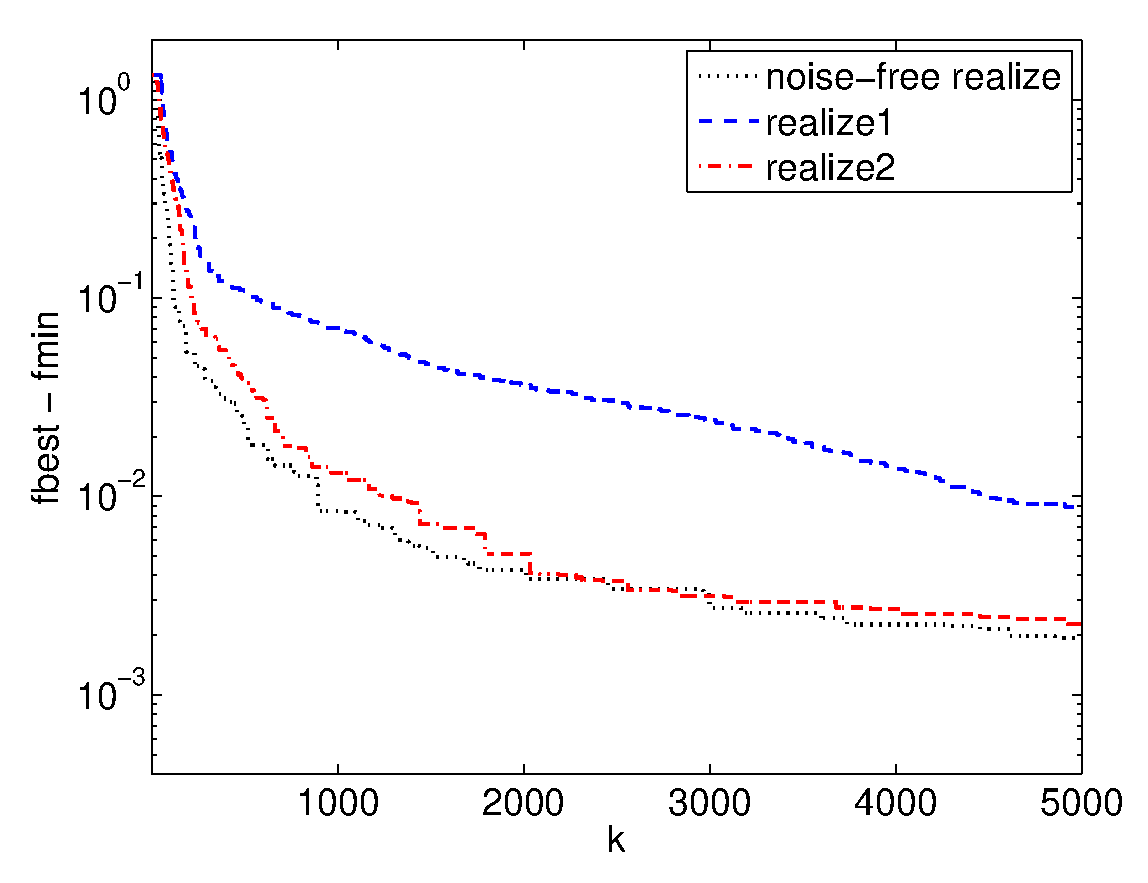
\includegraphics[width=0.65\textwidth]{matlab/pwl_error_fbest_realize}
\end{center}

\newpage

average and one std.\ dev.\ for
$f_\mathrm{best}^{(k)} - f^\star$
over $100$ realizations

\vfill

\begin{center}
\psfrag{k}[t][b]{$k$}
\psfrag{average fbest - fmin}[b][t]
{$\Expect f_\mathrm{best}^{(k)} - f^\star$}
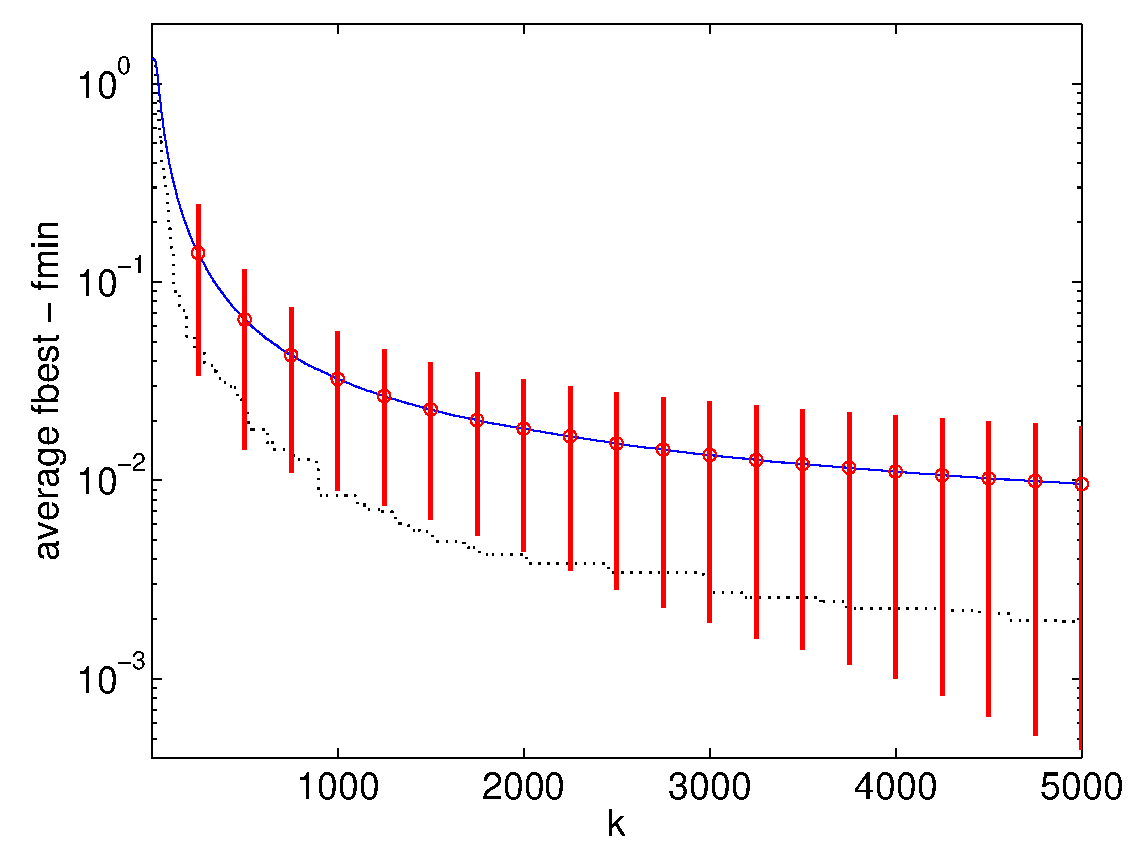
\includegraphics[width=0.65\textwidth]{matlab/pwl_error_fbest_average}
\end{center}

\newpage

empirical distributions of
$f_\mathrm{best}^{(k)} - f^\star$
at $k=250$, $k=1000$, and $k=5000$

\vfill

\begin{center}
\psfrag{iter 250}[c][b]{$k=250$}
\psfrag{iter 1000}[c][b]{$k=1000$}
\psfrag{iter 5000}[c][b]{$k=5000$}
\psfrag{average fbest - fmin}[b][t]
{$\Expect f_\mathrm{best}^{(k)} - f^\star$}
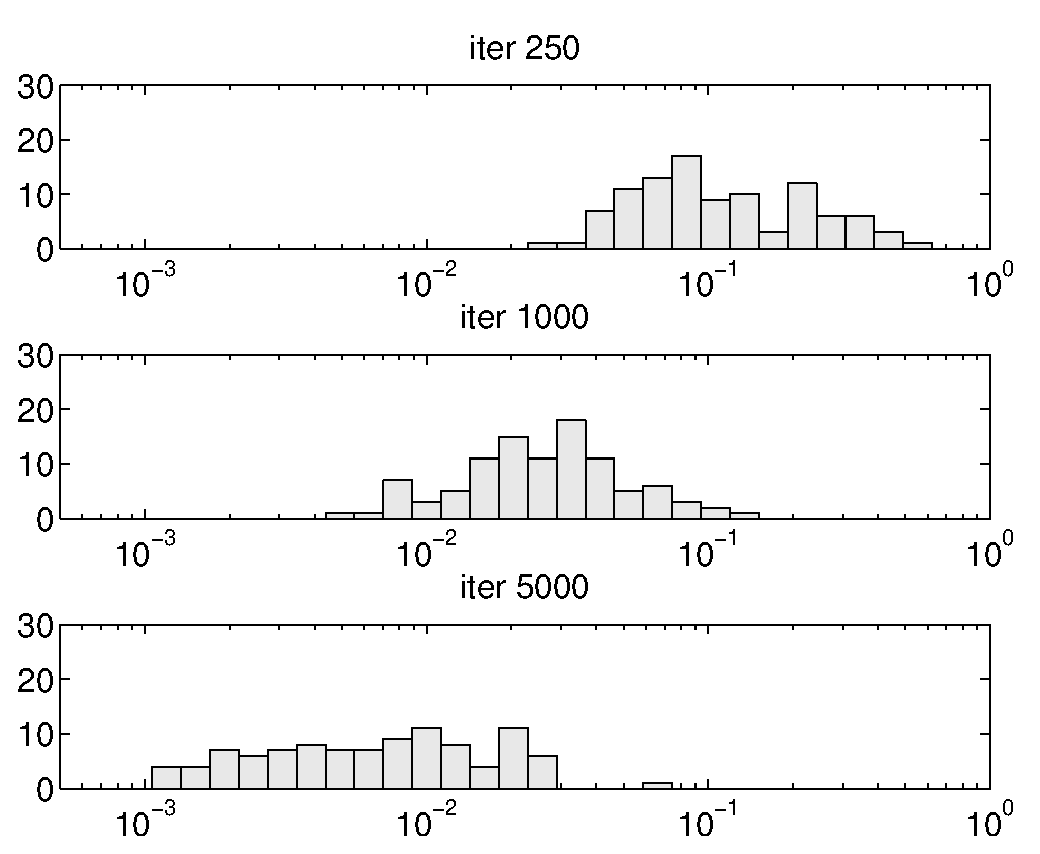
\includegraphics[width=0.65\textwidth]{matlab/pwl_error_fbest_dist}
\end{center}

\oursection{Stochastic programming}

\[
\begin{array}{ll}
\mbox{minimize} & \Expect f_0(x,\omega)\\
\mbox{subject to} & \Expect f_i(x,\omega) \leq 0, \quad i=1, \ldots, m
\end{array}
\]

if $f_i(x,\omega)$ is convex in $x$ for each $\omega$,
problem is convex

\vfill

`certainty-equivalent' problem
\[
\begin{array}{ll}
\mbox{minimize} & f_0(x, \Expect \omega)\\
\mbox{subject to} & f_i(x, \Expect \omega) \leq 0,
\quad i=1, \ldots, m
\end{array}
\]
(gives a lower bound on optimal value of stochastic problem)

\oursection{Variations}
\vfill
\BIT
\item
in place of $\Expect f_i(x,\omega)
\leq 0$ (constraint holds in expectation) can use
\BIT
\item $\Expect f_i(x,\omega)_+ \leq \epsilon$
(LHS is expected violation)
\item $\Expect \left( \max_i f_i(x,\omega)_+ \right) \leq \epsilon$
(LHS is expected worst violation)
\EIT
\item unfortunately, \emph{chance constraint}
$\Prob (f_i(x,\omega)\leq 0) \geq \eta$
is convex only in a few special cases
\EIT
\vfill



\oursection{Expected value of convex function}

suppose $F(x,w)$ is convex in $x$ for each $w$
and $G(x,w) \in \partial_x F(x,w)$
\BIT \itemsep -2pt
\item
$\displaystyle f(x) = \Expect F(x, w) = \int F(x,w) p(w) \; dw$
is convex
\item a subgradient of $f$ at $x$ is
\[
g=\Expect G(x,w) = \int G(x,w) p(w) \; dw \in \partial f(x)
\]
\item a noisy unbiased subgradient of $f$ at $x$ is
\[
\tilde g = \frac{1}{M} \sum_{i=1}^M G(x,w_i)
\]
where $w_1, \ldots, w_M$ are $M$ independent samples
(Monte Carlo)
\EIT

\oursection{Example: Expected value of piecewise linear function}


\[
\begin{array}{ll} \mbox{minimize} &
f(x) = \Expect\, \max_{i=1,\ldots,m} (a_i^T x + b_i)
\end{array}
\]
where $a_i$ and $b_i$ are random

\vfill

evaluate noisy subgradient using Monte Carlo method with
$M$ samples, and run stochastic subgradient method

\vfill
\vfill

compare to:
\BIT
\item certainty equivalent:
$
\mbox{minimize} \;
f_\mathrm{ce} (x) =
\max_{i=1,\ldots,m} (\Expect a_i^T x +  \Expect b_i)
$

\item heuristic:
$
\mbox{minimize} \; f_\mathrm{heur} (x) =
\max_{i=1,\ldots,m} (\Expect a_i^T x +  \Expect b_i
+ \lambda \|x\|_2)
$
\EIT

\newpage
problem instance:
$n=20$, $m=100$,
$a_i \sim \mathcal{N}(\bar a_i, 5 I)$,
$b \sim \mathcal{N}(\bar b, 5 I)$, \\
$\|a_i\|_2 \approx 5$, $\|b\|_2 \approx 10$,
$x_\mathrm{stoch}$ computed using $M = 100$

\vfill

\begin{center}
\psfrag{nominal}[c][b]{$x_\mathrm{ce}$}
\psfrag{heuristic}[c][b]{$x_\mathrm{heur}$}
\psfrag{K = 100}[c][b]{$x_\mathrm{stoch}$}
\psfrag{nom mean}{\small $f(x_\mathrm{ce})$}
\psfrag{nom nom}{}
\psfrag{heur mean}{\small $f(x_\mathrm{heur})$}
\psfrag{heur nom}{}
\psfrag{k100 mean}{\small $f(x_\mathrm{stoch})$}
%\psfrag{k100 mean}{}
%\psfrag{k100 nom}{$f_\mathrm{ce}(x_\mathrm{stoch})$}
\psfrag{k100 nom}{}
\psfrag{average fbest - fmin}[b][t]
{$\Expect f_\mathrm{best}^{(k)} - f^\star$}
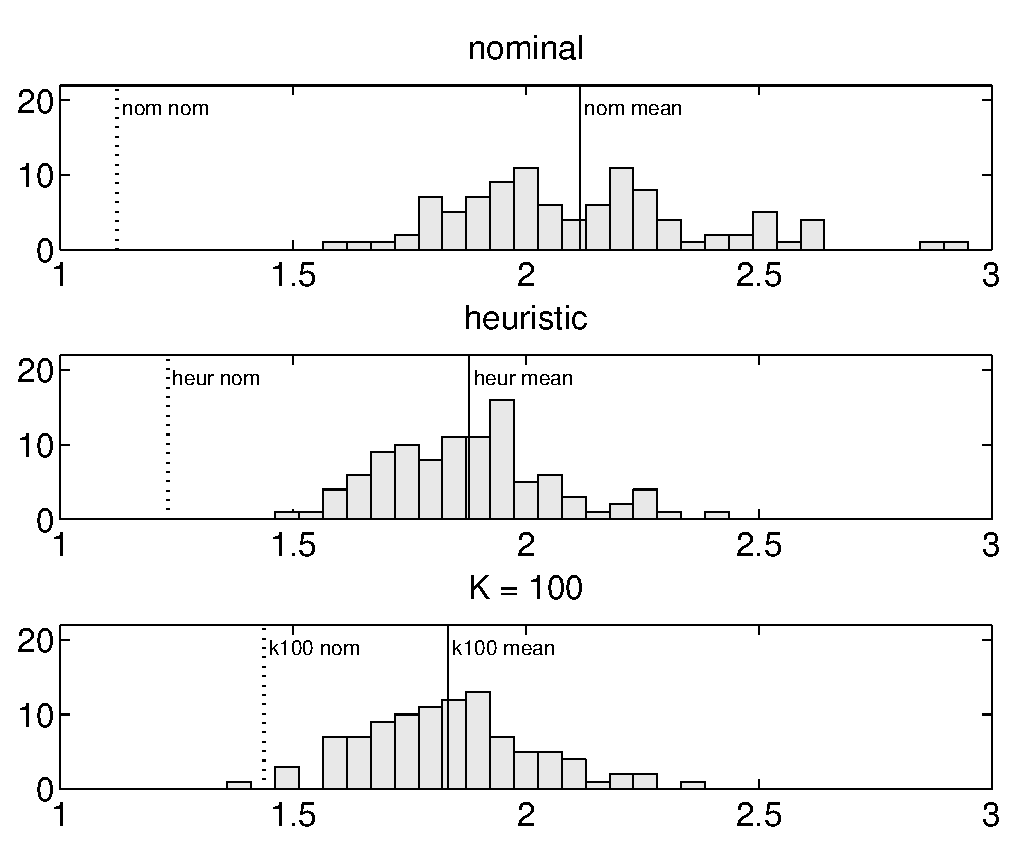
\includegraphics[width=0.65\textwidth]{matlab/expected_pwl_fbest_dist}
\end{center}

\newpage
$f^\star \approx 1.34$ estimated by running the method
with $M = 1000$ for long time

\vfill

\begin{center}
\psfrag{k}[t][b]{$k$}
\psfrag{fbest - fmin}[b][t]{$f_\mathrm{best}^{(k)} -\hat f^\star$}
\psfrag{K = 1}{\small $M=1$}
\psfrag{K = 10}{\small $M=10$}
\psfrag{K = 100 label}{\small $M = 100$}
\psfrag{K = 1000}{\small $M = 1000$}
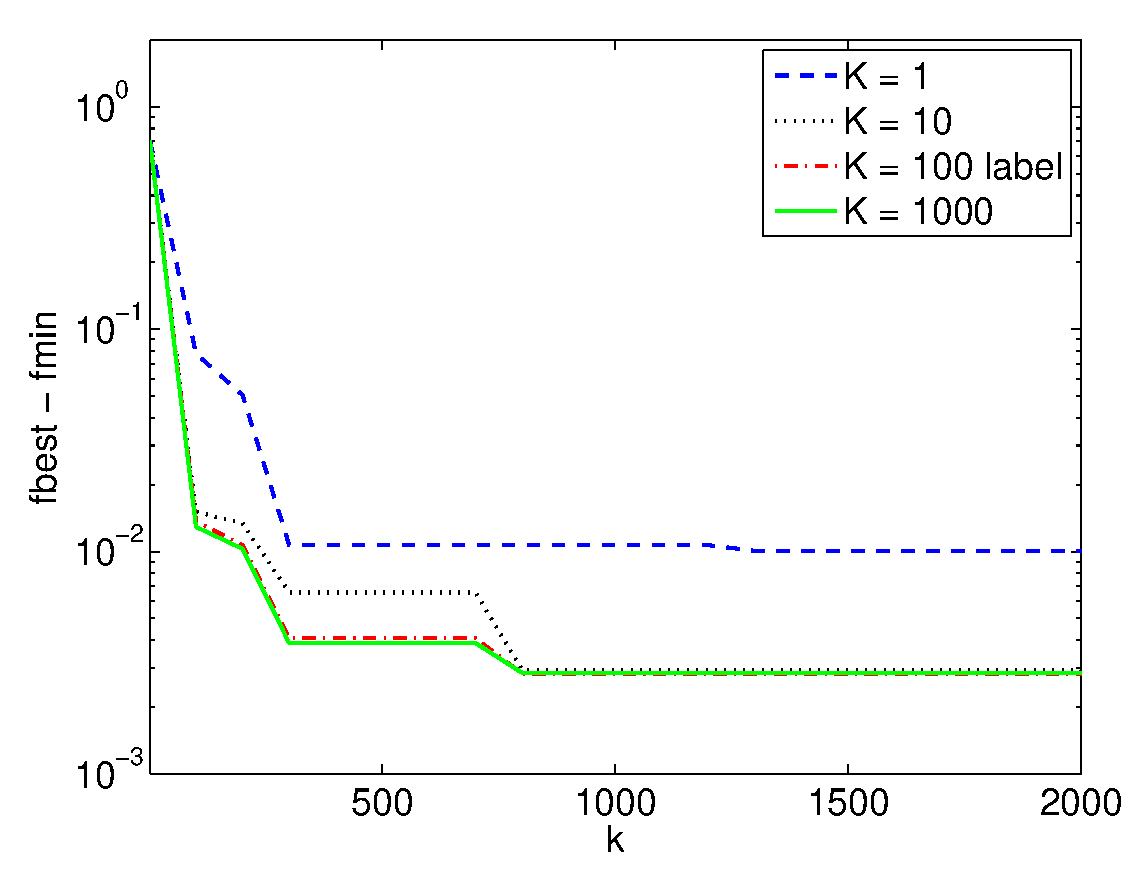
\includegraphics[width=0.7\textwidth]{matlab/expected_avgpwl_fbest}
\end{center}

\oursection{On-line learning and adaptive signal processing}

\BIT
\item $(x,y) \in \reals^n \times \reals$ have
some joint distribution
\item find weight vector $w \in \reals^n$ for which
$w^Tx$ is a good estimator of $y$
\item choose $w$ to minimize expected value
of a convex \emph{loss function} $l$
\[
J(w) = \Expect l(w^Tx-y)
\]
\BIT
\item $l(u)=u^2$: mean-square error
\item $l(u)=|u|$: mean-absolute error
\EIT
\item at each step (\eg, time sample), we are
given a sample $(x^{(i)},y^{(i)})$ from the distribution
\EIT

\newpage
noisy unbiased subgradient of $J$ at $w^{(k)}$, based on
sample $x^{(k+1)},y^{(k+1)}$:
\[
g^{(k)} = l'(w^{(k)T}x^{(k+1)}-y^{(k+1)})x^{(k+1)}
\]
where $l'$ is the derivative (or subgradient) of $l$

\vfill

on-line algorithm:
\[
w^{(k+1)}=w^{(k)}-\alpha_k
l'(w^{(k)T}x^{(k+1)}-y^{(k+1)})x^{(k+1)}.
\]

\BIT \itemsep -2pt
\item for $l(u)=u^2$, gives the LMS
(least mean-square) algorithm
\item for $l(u)=|u|$, gives the \emph{sign} algorithm
\item $w^{(k)T}x^{(k+1)}-y^{(k+1)}$ is the prediction error
\EIT

\oursection{Example: Mean-absolute error minimization}
problem instance: $n=10$, $(x,y) \sim \mathcal N(0,\Sigma)$,
$\Sigma$ random with $\Expect( y^2 ) \approx 12$, \\
$\alpha_k = 1/k$
\vfill

\begin{center}
\psfrag{pred error}[b][t]{prediction error}
\psfrag{k}[t][b]{$k$}
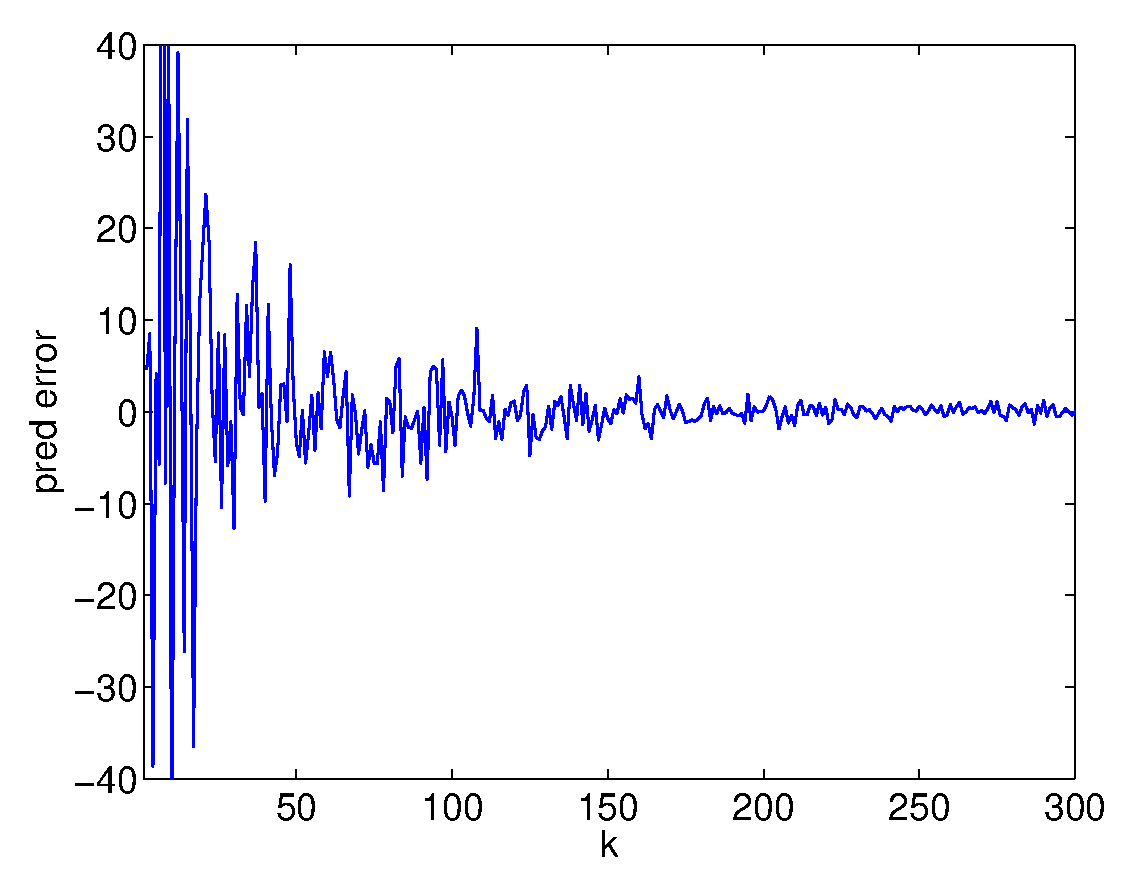
\includegraphics[width=0.6\textwidth]{matlab/online_reg_errors}
\end{center}

\newpage

empirical distribution of prediction error for
$w^{\star}$ (over $1000$ samples)

\vfill

\begin{center}
\psfrag{sign}[][]{}
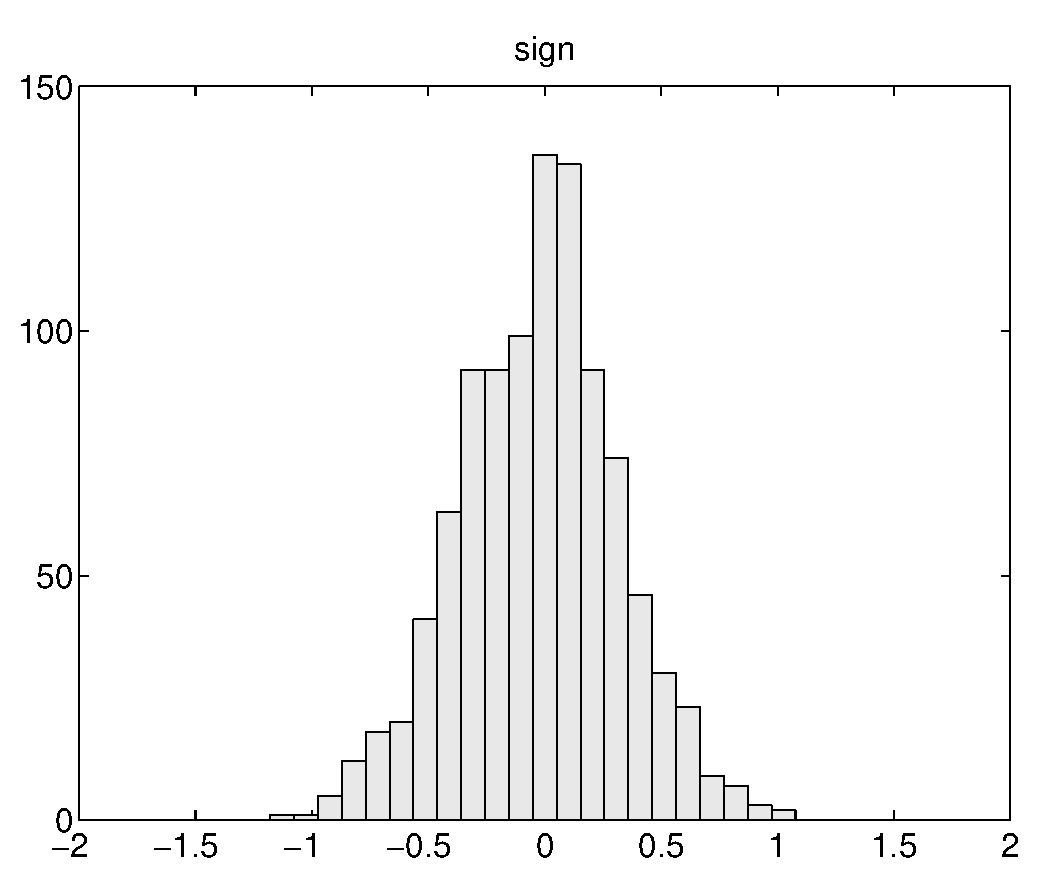
\includegraphics[width=0.65\textwidth]{matlab/online_reg_dist}
\end{center}

\end{document}
